\documentclass[a4paper]{article}
\usepackage{float}

%% Language and font encodings
\usepackage[english]{babel}
\usepackage[utf8x]{inputenc}
\usepackage[T1]{fontenc}
\usepackage{ae,aecompl,amsmath,amssymb,latexsym,fancyhdr,setspace}
%% Sets page size and margins
\usepackage[a4paper,top=3cm,bottom=2cm,left=3cm,right=3cm,marginparwidth=1.75cm]{geometry}

%% Useful packages
\usepackage{amsmath}
\usepackage{graphicx}
\usepackage[colorinlistoftodos]{todonotes}
\usepackage[colorlinks=true, allcolors=blue]{hyperref}
\title{Algoritmos}
\author{David Fernando Guerrero Alvarez}
\date{September 2018}

\begin{document}

\maketitle

\section{Taller #1}
1) Using Figure 2.2 as a model, illustrate the operation of INSERTION-SORT on the
array A =  \big \langle 31, 41, 59, 26, 41, 58 \big \rangle .\[\]\begin{figure}[H]
\centering
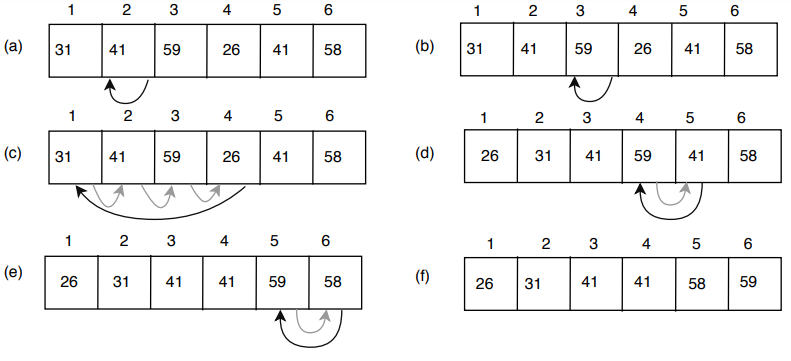
\includegraphics[width =1.0\textwidth]{Algo.PNG}
\end{figure}
\[\]2) Rewrite the INSERTION-SORT procedure to sort into nonincreasing instead of nondecreasing order. 
\begin{verbatim}
def insertionSortInverse(array):
   for i in range(1,len(array)):   
       aux = array[i]
       j = i - 1        
       while j > -1 and aux > array[j]:
           array[j + 1] = array[j]     
           j = j - 1
       array[j + 1] = aux

In: [5, 4, 6, 3, 7, 2, 8, 1, 9]
Out: [9,8,7,6,5,4,3,2,1]
\end{verbatim}
3) Consider the \textit{\textbf{searching problem}}:

\textbf{Input}: A sequence of n numbers A = \big \langle  \textit{a1, a2,..., an} \big \rangle and a value \textit{v}.

\textbf{Output}: An index \textit{i} such that \textit{v} = \textit{A[i]} or the special value NIL if \textit{v} does not appear in \textit{A}.

Write pseudocode for \textbf{\textit{linear search}}, which scans through the sequence, looking for \textit{v}. Using a loop invariant, prove that your algorithm is correct. Make sure that your loop invariant fulfills the three necessary properties. 
\begin{verbatim}
Programa: Búsqueda secuencial
Variables
T=10:entero
A[T]:arreglo de tamaño t
temp,i,j,n:entero
x:binario
Inicio
  //LLenar arreglo
  para i=0 hasta i< T incremento 1 hacer
    A[i]=númeroaleatorio
  fin para
  //Busqueda lineal
  leer n
  x=falso
  para i=0 hasta i< T incremento 1 hacer
    si A[i] = n entonces
      escribir "Valor encontrado"
      escribir "Posición:”, i
      x=verdadero
    fin si
  fin para
  si x=falso entonces
    escribir “No se encontró el número”
  fin si
Fin
\end{verbatim}
\textbf{Inicializacion:}
Se  inicia llenando un arreglo de tamaño T=10 con valores aleatorios luego se lee el valor a buscar y se compara este valor con el valor en la posicion inicial del arreglo.\\\\
\textbf{Mantenimiento:}
Se compara el valor obtenido al inicio con el siguiente término del arreglo A[i+1], repitiendo uno a uno el proceso de manera secuencial, si se encuentra que los terminos son iguales se cambia el valor de x de falso a verdadero y se escribe "valor encontrado" junto con su posicion en el arreglo y el algoritmo continúa. \\\\
\textbf{Terminacion:}\\
El algoritmo finaliza cuando ha recorrido cada uno de los elementos del arreglo i = T+1, si no encontro ninguna coincidencia entre el valor Inicial y los valores del arrelgo entonces x = falso y escribe "No se encontro el número".
\[\]
4)
Consider the problem of adding two n-bit binary integers, stored in two n-element arrays A and B. The sum of the two integers should be stored in binary form in an (n+1)-element array C. State the problem formally and write pseudocode for adding the two integers.\\\\
Declaration of A, B and C:\\\\
A[0] … A[n-1] (length = n)\\
B[0] … B[n-1] (length = n)\\
C[0] ... C[n] (length = n+1)\\
A[0] and B[0] are the most significant bits.\\\\
Pseudocode:\\

\begin{verbatim}
Carry = 0
For i = n - 1 to 0
    C[i+1] = (A[i] + B[i] + Carry) mod 2
    Carry = (A[i] + B[i] + Carry) / 2
C[0] = Carry
\end{verbatim}
 
\end{document}